\documentclass[conference]{IEEEtran}
\IEEEoverridecommandlockouts
% The preceding line is only needed to identify funding in the first footnote. If that is unneeded, please comment it out.
\usepackage{cite}
\usepackage{amsmath,amssymb,amsfonts}
\usepackage{algorithmic}
\usepackage{graphicx}
\usepackage{textcomp}
\usepackage{xcolor}
\def\BibTeX{{\rm B\kern-.05em{\sc i\kern-.025em b}\kern-.08em
    T\kern-.1667em\lower.7ex\hbox{E}\kern-.125emX}}
    
\makeatletter
\def\endthebibliography{%
  \def\@noitemerr{\@latex@warning{Empty `thebibliography' environment}}%
  \endlist
}
\makeatother    
    
\begin{document}

\title{Precise ECG Platform on Modern Processors}

\author{\IEEEauthorblockN{S. Normalized Infloop}
\IEEEauthorblockA{\textit{Department of Calculator Science} \\
\textit{Theoretical Abstract Interpretation Testing Society}\\
Pitsston, PA, United State Monads of America \\
\texttt{yueyao@andrew.cmu.edu}}
\and
\IEEEauthorblockN{2\textsuperscript{nd} Given Name Surname}
\IEEEauthorblockA{\textit{dept. name of organization (of Aff.)} \\
\textit{name of organization (of Aff.)}\\
City, Country \\
email address}
}

\maketitle

\begin{abstract}
The authors shivers in the howling wind on Pausch Bridge, wondering why the processors in their backpacks gets to sit comfortably and doing nothing instead of switching their tiny transistors to keep their owners, who paid BIG money to buy them, warm. 
\end{abstract}

\begin{IEEEkeywords}
Thermal Systems, Ambient Heat Modulating Technologies, Parallel Heating, 2D Computer Graphics, Edible Content Generation
\end{IEEEkeywords}

\section{Introduction}

Of all the things computing machines brought to the world, there is one thing that people 
have consistently tried hard to get rid of since the dawn of this field. Dissipating heat
in computing system has become a major design problem in all levels of computer engineering. 
Modern processors is on the verge of, if not already, hitting on one of the major design 
boundaries known as the power wall (the chip’s overall temperature and power consumption)~\cite{patterson2006future}. 
Some people believe that ``the power wall is now arguably the defining limit of the power 
of the modern CPU"\cite{mims2010}.

If we are unable to curse of this everyday intensifying brownian motion within the computing
machines, why not take advantage of it? Heat, as a resource, can be very useful in a number of ways.
In fact, heat is a very important resource widely used in \textit{Edible Content Generation (ECG)} process. 
Edible Content Generation takes (usually) biological specimens and apply a sequence of chemical and physical
decorations to them, generating human digestible contents. This process is more commonly known as \textit{cooking}.

It has been over a decade since people has tried to utilize the heat generated from computing
devices to facilitate ECG. However, a vast majority of those attempts has failed and results in
either overheated computing devices or unsuccessful ECG process. The authors believe the problem is
that operators of such process have very little control on the power of the heating device, compared to
tradition ECG platforms (more commonly known as stoves). This work addresses this problem by proposing
a way to turn modern processors into precise ECG platforms, which users have precise control of power down
to every second.

\section{Computing Device Based ECG Platforms}

\subsection{Graphics Device Based ECG Platforms}

\section{System Architecture}
The goal of this work is to implement a precise ECG platform on a modern processor. 
Modern processors refers to processors with many cores and possibly SMT support. By
saying precise we wish to grant users very fined grained control of ECG platform power
output for every second. Controlling power consumption of processors roughly translates
into controlling CPU utilization rate \cite{fan2007power}. In conclusion, we need to
design a system that gives user control on CPU utilization, down to every second, on 
modern multi-core processors. 

The code for this work is available on GitHub at \texttt{https://github.com/codeworm96/heat}.

\subsection{Load generation by frequency modulation.}
\begin{figure}[htbp]
\centerline{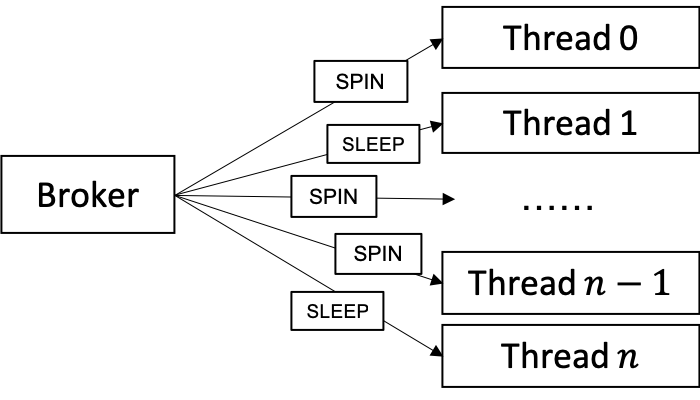
\includegraphics[scale=.5]{fig/broker.png}}
\caption{Broker dispatches tiny chunk of work to threads.}
\label{arch}
\end{figure}

Our system is built upon a standard broker-worker architecture. A globally shared broker
will generate work for each thread. Each thread independently obtains jobs from the broker, 
executes it, and starts over. There are two types of jobs:

\begin{itemize}
\item \textbf{SLEEP}. The thread will sleep for a small period of time.
\item \textbf{SPIN}. The thread will spin in a tight loop for a small period of time.
\end{itemize}

Usually the size of both jobs is set to $1~\textrm{ms}$. The broker randomly generates jobs
based on a desired system load. For example, if the desired CPU utilization is 10\%, the 
broker has a 1/10 probability of generating a \texttt{SPIN} work. It should be self evident
that this strategy indeed achieves the required CPU utilization. The proof is left as an exercise
for the reader. Essentially this scheme achieves a certain system load by modulating 
frequency of processor spinning. This scheme is thus termed (job) frequency modulation. The
probability of generating a spin job is termed \textit{spin rate}, denoted by $s$.

This scheme is better than the length modulation scheme, where we adjust the length of 
spinning jobs relative to sleep job. Frequency modulation provides a more stable CPU
load over time (less variation in utilization). For every (large enough) time window, 
the average CPU utilization will be identical regardless where the window is. On the other
hand, frequency modulation helps to achieve precise control of CPU utilization.

\subsection{Load compensation by PI controller.}
It is often the case where people need to work while using ECG platforms. This causes the
problem if the user is working on the computing device while its being used as an ECG platform.
The workload generated by the user will very likely affect overall CPU utilization and increase
power output, which may overcook edible contents, or worse, destroys the device. It is essential
for the ECG platform to be able to compensate for the load. 

Due to the unpredictable nature of the user workload, it will be very hard to model (even reliably measure) 
user workload online. Here we took a feedback control system approach. We attach what is known as an 
\textit{proportionate-integral controller} (PI controller) to the output. For those unfamiliar with the 
concept, we provide the following explanation. 

For every time step, there exists a desired CPU utilization $L_0$. It also measures the current CPU utilization, 
which denoted as $L$. The error $e$ as this time step is defined as $e \triangleq L - L_0$. Clearly $e$ is a function
of time $t$, The compensation factor $s'$ is calculated as
$$ s' \triangleq P~e(t) + I\int_{0}^{t}e(t)~dt$$
where $P$ and $I$ are two coefficients termed proportionate coefficient and integral coefficient. Finally, if the spin
rate dictated by desired CPU utilization is $s_0$, then the actual spin rate used by the broker will be $s = s_0 + s'$.

Intuitively, the $P$-term compensates for sudden changes in user load, while the
$I$-term compensates for long running user load. To ensure negative feedback, both $P$ and $I$ must be negative.

\subsection{Intuitive load specification.}

Our proposed ECG system features a very intuitive way for the user to specify the desired load. 
Since many users of ECG systems are not tech-savvy, it's very important to keep the interface simple. 
The users of our system may specify a ``program" by supplying a textual file, whose contents mimics the
desired shape of CPU utilization graph (except the time is the Y axis). 

For example, the following config file specifies that the system should run a loop that utilization is
40\%, 80\%, 20\%, 70\%  for the first, second, third, and fourth second of each iteration.

\begin{verbatim}
||||
||||||||
||
|||||||
\end{verbatim}

This interface is intuitive and very easy to use. It is so simple that only one character is involved, and
no formal specification or documentation is needed to understand this format. We name this form \texttt{YAMMY} as in
\textit{\textbf{Y}et \textbf{A}nother \textbf{M}arkup-lang? \textbf{M}y \textbf{G}od!} format. The authors are 
convinced that this format will be as popular in the field of ECG platform research as JSON in machine learning research.

\section{Results}

We implemented our work and tested the work on one of GHC machines. Unfortunately the authors are denied physical access to
GHC machines the moment the told the administration staff that want to perform ECG experiment on one of their computers. The 
authors have no idea why the administration staff holds such hostility to legit scientific research and edible contents. The 
best we have is running our program while monitoring CPU utilization. 

As you can see, our results proves the effectiveness of our approach.

\section{Conclusion}

Since the authors are denied physical access to GHC machines, the authors believes there is no future of ECG platform research
unless administration staff stop discriminating ECG platform researchers. Whats the point of doing ECG research when you cannot
conduct proper ECG experiments? This field is DOOMED, dude! Get out! Learn you a Haskell for greater good~\cite{harper2016practical}. 


\ifCLASSOPTIONcaptionsoff
  \newpage
\fi
\bibliographystyle{IEEEtran}
\bibliography{ref}

\end{document}
